\begin{figure}[tb!]
	\centering
	\begin{subfigure}[b]{0.45\textwidth}
		\centering
		\begin{tikzpicture}
			
			[
				level distance=24pt,
				every tree node/.style={align=center,anchor=base},
				frontier/.style={distance from root=92pt},
				edge from parent/.style={draw,edge from parent path={(\tikzparentnode.south) {[rounded corners=0.5pt]-- ($(\tikzchildnode |- \tikzparentnode.south) + (0, -5pt)$) -- (\tikzchildnode)}}}
			]
			\Tree
			[.S
				[.NP I$_1$ ]
				[.ADVP really$_2$ ]
				[.VP love$_3$ [.NP this$_4$ game$_5$ ] ]
			];
		\end{tikzpicture}
		\caption{原始句法树}
		\label{fig:con-original-tree}
	\end{subfigure}
	\hfill
	\begin{subfigure}[b]{0.45\textwidth}
		\centering
		\begin{tikzpicture}[
				level distance=24pt,
				every tree node/.style={align=center,anchor=base},
				frontier/.style={distance from root=92pt},
				edge from parent/.style={draw,edge from parent path={(\tikzparentnode.south) {[rounded corners=0.5pt]-- ($(\tikzchildnode |- \tikzparentnode.south) + (0, -5pt)$) -- (\tikzchildnode)}}}
			]
			\Tree
			[.S
				[.$\textrm{S}^\ast$ [.NP I$_1$ ] [.ADVP really$_2$ ] ]
				[.VP
					[.$\textrm{VP}^\ast$ love$_3$ ]
					[.NP [.$\textrm{NP}^\ast$ this$_4$ ] [.$\textrm{NP}^\ast$ game$_5$ ] ]
				]
			];
		\end{tikzpicture}
		\caption{遵循乔姆斯基范式的左二叉化句法树}
		\label{fig:con-binaried-tree}
	\end{subfigure}
	\caption{
		成分句法树的例子.
		其中词性在这里被忽略
	}
	\label{fig:con-tree-full-figure}
\end{figure}
